\section{CV17 with Independent Calibration}
\label{sec:cv17}
CV17 supplies a higher-utility teacher regime with independent health calibration. Data, optimization, noise, routing, and comparisons were fixed before teacher training/test evaluation. This separate protocol does not reconstruct the earlier manuscript's unavailable partition.

\subsection{Data, Optimization, and Paired Controls}
\label{sec:cv17_protocol}
\paragraph*{Fixed data and speaker separation}
The English CV17 mirror (revision \texttt{8262c16}, CC0-1.0)\footnote{\url{https://huggingface.co/datasets/fsicoli/common_voice_17_0}; pinned third-party mirror.} supplies England/British, Indian/South Asian and US accents (Table~\ref{tab:app_data_stats}). Source-compatible TSV parsing uses \texttt{csv.QUOTE\_NONE}. Of 445,742 eligible rows, shuffling and capping at 20 clips/client (seed 20260908), then sampling (20260909), yields the training corpus.

Class-stratified client splitting of 1,458 development clips (seed 20260910) separates selection and calibration. Client and clip IDs are pairwise disjoint across all four sets; client IDs proxy speakers. Seeds 0--9 reserve $1/4$ of training clients for auxiliary learning, measuring partition/optimization variation on this fixed corpus.

\begin{table}[t]
\centering\scriptsize\setlength{\tabcolsep}{3.4pt}
\caption{CV17 client-disjoint corpus counts.}
\label{tab:app_data_stats}
\begin{tabular}{lrrrrr}\toprule
Split & Clips & England & Indian & US & Clients\\\midrule
\csname @@input\endcsname{restored_tables/data_stats.tex}
\bottomrule\end{tabular}
\end{table}

Seed 0 has 37,462/12,538 private/auxiliary clips, with class counts $(7,228,5,676,24,558)$ and $(2,496,1,554,8,488)$. All seed-wise partitions are saved. Calibration assesses the selected teacher on a different speaker group without consulting test outcomes.

\paragraph*{Features and optimization budget}
The pinned IV-A encoder successfully processes all 53,133 clips: mono 16~kHz, 12-second truncation, real-waveform normalization, fixed zero padding to 12 seconds, and mean pooling over valid final-layer frames. Fixed padding removes batch-composition dependence. Each seed fits an auxiliary-only standardizer, then unit $\ell_2$ normalization. Teacher/student heads are linear $768\to3$.

Teachers/students use 80 epochs, AdamW learning rate 0.03, weight decay $10^{-4}$, and batch 256, following a development-only non-DP check on IV-A's different archive. DP BS uses auxiliary counts, $C=2$, and $\sigma=0.5,1,2,4,8$. Unit features bound the full linear CE/BS gradient (including bias) by 2. Controls are non-DP CE/BS and DP CE at $\sigma=1$. Maximum selection Macro-F1 chooses checkpoints, earliest on ties; calibration never selects.

Private sizes 37,333--37,705 give Poisson $q=1/146,1/147,1/148$ and 11,680--11,840 updates. Opacus 1.6 PRV accounts for all 80 epochs, with tolerances 0.01 in $\varepsilon$ and $\delta/1000$ at $\delta=10^{-5}$. Each bound protects one head-training condition, not encoder pretraining, auxiliary data or a joint release of all teachers. Public-benchmark seeds aid reproduction; private deployment needs undisclosed noise and composition of all inspected runs.

\paragraph*{Attenuation and routing controls}
Each DP BS teacher supplies KD, instance/class/confidence HAKD, global-T CTKD and mean-matched KD students. Hard is shared across noise settings within seed; initialization/order use $s+1000003$/$s+1000004$. KD uses $\alpha=0.7,T=2$; CTKD retains its published mechanism and ten-epoch ramp. Uniform HAKD equals KD at loss/gradient level and reuses its run. There are 80 teachers and 310 students.

Mean-matched KD uses constant KL/CE weights $(\alpha\bar w,1-\alpha\bar w)$, where $\bar w$ averages~\eqref{eq:hakd_weight} over auxiliary examples using the same teacher/calibration recalls. It isolates average attenuation from instance variation. TCRD/RC retain equal weights and $(0.45,0.60)$; binary T-BAcc retains 0.45. Three-way $B$-only routing uses both TCRD thresholds. S-BAcc selects Hard/KD/HAKD on selection BalAcc, ties in that order.

\subsection{Teacher and Student Outcomes}
\label{sec:cv17_outcomes}
\begin{table}[t]
\centering\scriptsize\setlength{\tabcolsep}{2pt}
\caption{CV17 teachers and calibration (ten seeds).}
\label{tab:cv17_teachers}
\begin{tabular}{lcccc}\toprule
Teacher & PRV $\varepsilon$ & BalAcc & MF1 & Health range\\\midrule
\csname @@input\endcsname{cv17_tables/teachers_compact.tex}
\bottomrule\end{tabular}
\end{table}

\begin{table*}[t]
\centering\scriptsize\setlength{\tabcolsep}{3pt}
\caption{CV17 paired students: BalAcc / Macro-F1, in percent (ten seeds).}
\label{tab:cv17_students}
\begin{tabular}{lccccc}\toprule
Mode & $\sigma=0.5$ & $\sigma=1$ & $\sigma=2$ & $\sigma=4$ & $\sigma=8$\\\midrule
\csname @@input\endcsname{cv17_tables/students_compact.tex}
\bottomrule\end{tabular}
\end{table*}

Table~\ref{tab:cv17_teachers} shows non-DP CE/BS BalAcc 0.701/0.729, with lower BS Macro-F1. DP BS/CE at $\sigma=1$ gives BalAcc 0.694/0.665 but Macro-F1 0.653/0.676. BS changes the precision--recall trade-off. Both corpus and optimization differ from IV-A, so this does not isolate data size.

In Table~\ref{tab:cv17_students}, KD-minus-Hard BalAcc gains across increasing $\sigma$ are $+4.47,+3.30,+1.51,-0.63,-4.07$ points, positive in $10/10/8/4/0$ seeds. Health 0.530--0.631 selects 24 KD and 26 HAKD branches, no Hard. The separate low-health studies in IV supply the exclusion cases.

Grid-averaged TCRD-minus-Hard BalAcc is $+2.20$ points (95\% paired seed interval $[1.53,2.81]$); gains over binary/three-way $B$ routes are $+1.29/+0.48$ (Table~\ref{tab:cv17_contrasts}). Macro-F1 versus Hard is $-0.28$ points ($[-0.80,0.24]$). Versus S-BAcc, BalAcc is $-0.21$ ($[-0.41,0.01]$) and Macro-F1 $-0.91$ ($[-1.19,-0.61]$): student validation remains competitive.

\paragraph*{What HAKD contributes}
Instance HAKD beats both Hard and KD in 35/50 conditions, with grid-mean BalAcc gains $+2.43/+1.51$ points. At $\sigma=8$, its mean BalAcc is 0.675 versus Hard's 0.679 and KD's 0.638: attenuation reduces but does not eliminate negative transfer. Versus mean-matched KD it differs by $-0.0016$ points ($[-0.17,0.18]$); Macro-F1 differs by $-0.023$ ($[-0.19,0.14]$). The evidence supports attenuation, not an instance-specific advantage. Class/confidence weights remain competitive.

\subsection{Incremental Value and Uncertainty}
\label{sec:cv17_incremental}
\paragraph*{Prespecified component and gain checks}
Components use equal weights, singles, leave-one-out averages, and permutations of $(0.5,0.25,0.25)$, distinct from VCTK's biased weights. Utilities reuse paired branches; H/A/K counts cover 50 conditions. Grid summaries first average five noises within seed, then summarize ten seeds; 95\% intervals use 20,000 paired seed resamples without multiplicity adjustment. These quantify run variation on fixed cohorts.

Leave-one-seed-out ridge regression (penalty 1) predicts KD-minus-Hard gain from $B$, $H$, or $(B,F,1-M)$. Standardization and fitting use the other nine seeds; held-out errors average each seed's five noises. This checks fixed-corpus prediction, not a test-trained policy.

Table~\ref{tab:cv17_components} shows changed routes without indispensable components: dispersion-only and leave-$B$-out always select HAKD, BalAcc 0.703 versus equal weights' 0.701. Health--gain Pearson/Spearman correlations are 0.858/0.857, versus $B$'s 0.872/0.881 (Fig.~\ref{fig:cv17_gain}). Useful routing and incremental gain prediction are distinct.

Held-out MSEs for $B/H$/all components are $3.06/3.35/3.47\times10^{-4}$. Composite-minus-$B$ MSE is $0.29\times10^{-4}$ (95\% seed interval $[-0.47,1.00]\times10^{-4}$); all-components-minus-$B$ is $0.41\times10^{-4}$ ($[0.012,0.95]\times10^{-4}$). Richer scores do not improve prediction; TCRD's routing gain concerns the specified score/threshold choices.

\begin{table}[t]
\centering\footnotesize\setlength{\tabcolsep}{3pt}
\caption{CV17 health-component ablations (ten seeds).}
\label{tab:cv17_components}
\begin{tabular}{lccc}\toprule
Weighting & H/A/K & BalAcc & Macro-F1\\\midrule
\csname @@input\endcsname{cv17_tables/components.tex}
\bottomrule\end{tabular}
\end{table}

\begin{table}[t]
\centering\footnotesize\setlength{\tabcolsep}{4pt}
\caption{CV17 paired BalAcc differences (percentage points; 95\% seed intervals).}
\label{tab:cv17_contrasts}
\begin{tabular}{lrc}\toprule
Comparison & Mean & Bootstrap 95\% interval\\\midrule
\csname @@input\endcsname{cv17_tables/contrasts.tex}
\bottomrule\end{tabular}
\end{table}

\begin{figure}[t]
\centering
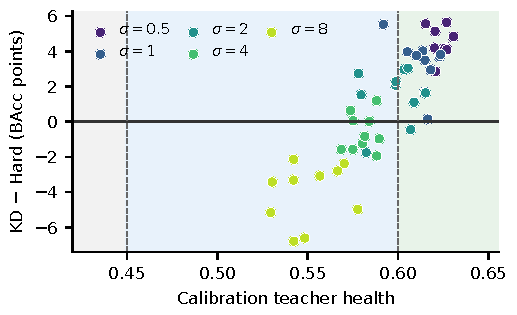
\includegraphics[width=\linewidth]{figure/cv17_health_gain.pdf}
\caption{CV17 calibration health versus paired KD gain.}
\label{fig:cv17_gain}
\label{fig:cv_health_vs_gain}
\end{figure}

\paragraph*{Independent calibration and speaker dependence}
For each selected teacher, 2,000 calibration-speaker bootstrap draws retain every utterance within sampled clusters. Their health SD enters the same Gaussian region rule; multinomial SE is the comparator. Test health is report-only, a noisy finite held-out proxy, not a population-coverage target.

Mean cluster SEs span 0.0185--0.0195 versus multinomial 0.0142--0.0148, changing 12/50 RC decisions. Cluster RC certifies 16 and falls back in 34, reducing BalAcc versus TCRD by 1.70 points ($[-2.16,-1.25]$); Macro-F1 changes $+0.10$ ($[-0.32,0.51]$). Deterministic/RC actions disagree with test-health regions in 15/36 cases; only two RC disagreements are certified. Nominal 95\% cluster intervals contain test-health points in 37/50 cases. Independent calibration removes same-set selection, not the distinction between region confidence and useful transfer.
